\section{Serverless Architecture}\label{sec:architecture}

The architecture 


l'architettura del sistema � serverless nel senso che non necessita la gestione da parte del ... di alcun server.

curare numerosi aspetti, integrando servizi di terze parti "as-a-Service"-like che adempiono e rimpiazzano codice "propietario"/specifico: distribuzione, user management, models generation, users collaboration, state storage

\subsubsection*{Distribution}

distribution of the web application => webserver => CDN (Akamai)

\subsubsection*{User Management}
user management => backend => Backend-as-a-Service (Auth0)

\subsubsection*{Model Generation}
3D model generation of heavy building elements => backend => Function-as-a-Service (AWS lambda)

\subsubsection*{Users Collaboration}
users collaboration => backend => Backend-as-a-Service (Firebase)

\subsubsection*{State Storage}
state storage =>  DB => Compose.io (DA VERIFICARE)

In particolare, la serializzazione/deserializzazione dello stato completo dell'applicazione � supportata da uno stato centralizzato.

L'architettura software del frontend � reactive => gli passo lo stato ottenuto dal server, aggiorna tutta l'interfaccia.

\iffalse
We used a Serverless Architecture to deploy all the work. L'intero sistema viene distribuito sfruttando sistemi "as-a-Service" come le CDN, BaaS e FaaS, delegando la gestione dell'infrastruttura hardware e di manutenzione ai rispettivi fornitori di servizi.
\fi

\iffalse
To offer the application to end-users with high availability and high performance we deployed all Javascript files that are part of the system into a CDN (Content Delivery Network). This single point of deploy offered us a centralized method to upgrade all customers applications without any customer explicit action.
\fi

To perform CPU intensive operations, necessary to make complex geometric element, we used a third party FaaS system that run Python functions and that generate 3D elements. Thank to this we can scale up and down and adjust the CPU load on the traffic.

The collaboration part is based on a DBaaS, with the common state stored in an external DB provided by Firebase. Following this methodology we could also add user authentication features based on external BaaS providing all user management functionalities.

The application is distributed as frontend web application and so it's mostly executed into customer's browser. The application state is inside the customer's browser and it is represented as a tree structured object. This state can be serialized and saved on a BaaS system or downloaded as JSON file. The customer can restore the application state in any time using a preceding downloaded serialized version of the state. The system will adjust the user interface and the scene by means of the Virtual DOM and the diff and patch algorithm. Il server quindi si rivela necessario solo nei rari casi in cui l'utente opta per un salvataggio online.


L'intero stato dell'applicazione completamente serializzabile come documento permette di eseguire la modellazione 2D all'interno del frontend e di contattare il server solamente per il salvataggio del dato. La serializzazione dello stato come JSON  abilita l'utilizzo di molteplici sistemi per il salvataggio dei dati, in quanto non viene richiesto un backend personalizzato, ma può esser utilizzato un qualsiasi DBaaS a patto che supporti il savataggio di JSON. Il progetto è stato realizzato connettendo i dati tramite Firebase.

%
% In Figure~\ref{fig_serverless} there is the architectural schema described above\\\\
% 
% \begin{figure}[htb]
% \centering
% 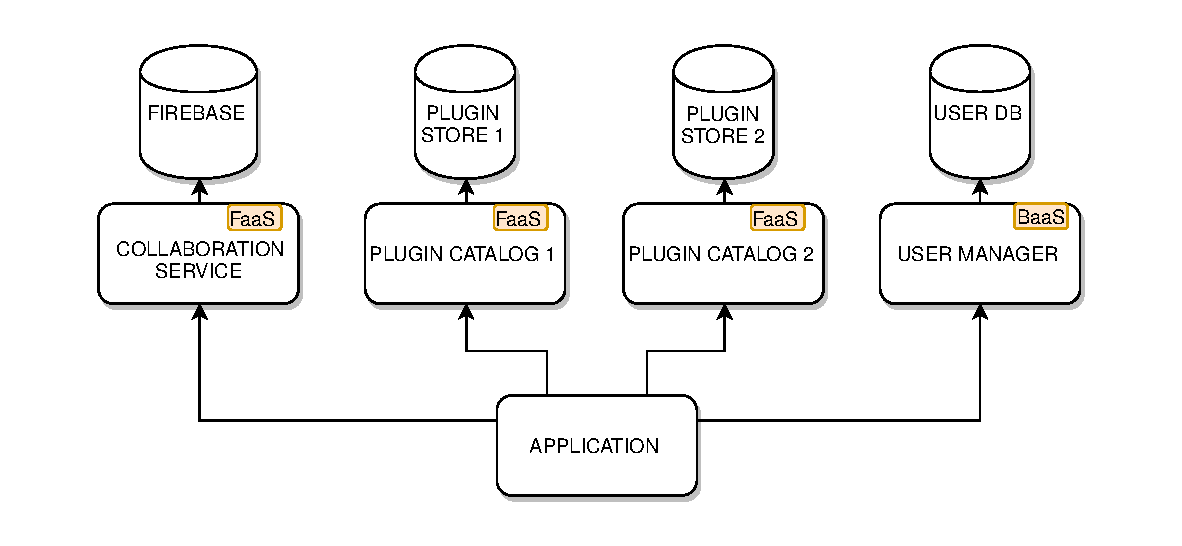
\includegraphics[width=\linewidth]{contents/images/serverless-diagram}
%
% \caption{The serverless architecture for our application.}
% \label{fig_serverless}
% \end{figure}


\subsection{Centralized Application State}\label{ssub:centr_state}

Per abilitare il supporto alla serializzazione del dato è necessario lavorare attraverso un unico stato centralizzato nel quale vengono memorizzate tutte le informazioni. Ciò è stato possibile utilizzando il pattern \textbf{unidirectional data flow pattern}.
Questa scelta ha anche portato dei benefici nell'architettura complessiva del sistema che può essere suddivisa in 3 macroblocchi: (i) la parte logica, (ii) la visualizzazione 2D (iii) la visualizzazione 3d. Un precedente esperimento di sviluppo di un progetto simile \footnote{https://github.com/cvdlab/walle} che non utilizzava questo approccio ha evidenziato un accoppiamento tra il motore logico e la UI. Lo sviluppo di una nuova funzionalità richiedeva anche lo sviluppo di procedure che attraverso listener aggiornavano l'interfaccia adeguandola al cambiamento.



The application exploits the \textbf{unidirectional data flow pattern} to gain great benefits in terms of maintainability of the software objects, due to the lightness of the resulting architecture. As requested by the pattern, the software has to be based on a \textbf{centralized state}, which represents the application logic. Consequently, every feature has as its unique goal the obtainment of a new state coherent with the requested change, following various mechanisms based on \textbf{actions} (each one containing the data for the new state) and \textbf{reducers} (software objects that can write the new state) provided by the \textbf{Redux.js}\footnote{http://redux.js.org/} library. Usually, the unidirectional data flow pattern is associated with the \textbf{Immutability pattern}, which contributes to maintainability, avoiding side effects for state changes and providing smaller tests for application logic changes. We also benefits of undo/redo operations to an oldest/newer state by means of a replace of the current state with the previous/next one. As a consequence, the state can be seen as an \textbf{immutable tree structure} whose changes require: (i) The build of a new state \texttt{s'} equal to the previous state \texttt{s}; (ii) Execution of changes on the new state \texttt{s'}; (iii) Reference replacement from \texttt{s} to \texttt{s'}. Despite its simplicity, this pattern can nevertheless lead to memory waste, so we used the \textbf{Immutable.js}\footnote{https://facebook.github.io/immutable-js/} library (made by facebook), which exploits structural sharing via hash maps tries and vector tries minimizing the need to copy or cache data.
In our application, the state contains all the parts that there are on a plan, giving life to a finite state machine of all possible evolutions of the application state, where each node correspond to a \textbf{mode} (and consequently to a possible application state), and each edge correspond to an action from that point (which in our case is typically a javascript event such as \texttt{click} or \texttt{mousemove}). A part of the state machine is shown in figure~\ref{fig_uc_draw_wall}. How we can see there are three nodes corresponding to three modes: (i) Node \texttt{idle}: waiting mode of the application. No action has been taken yet. (ii) Node \texttt{waiting\_drawing\_wall}: user has selected wall design tool, but he hasn't started the draw phase yet. (iii) Node \texttt{drawing\_wall}: user has placed the starting point of the wall.

\begin{figure}[!t]
\centering
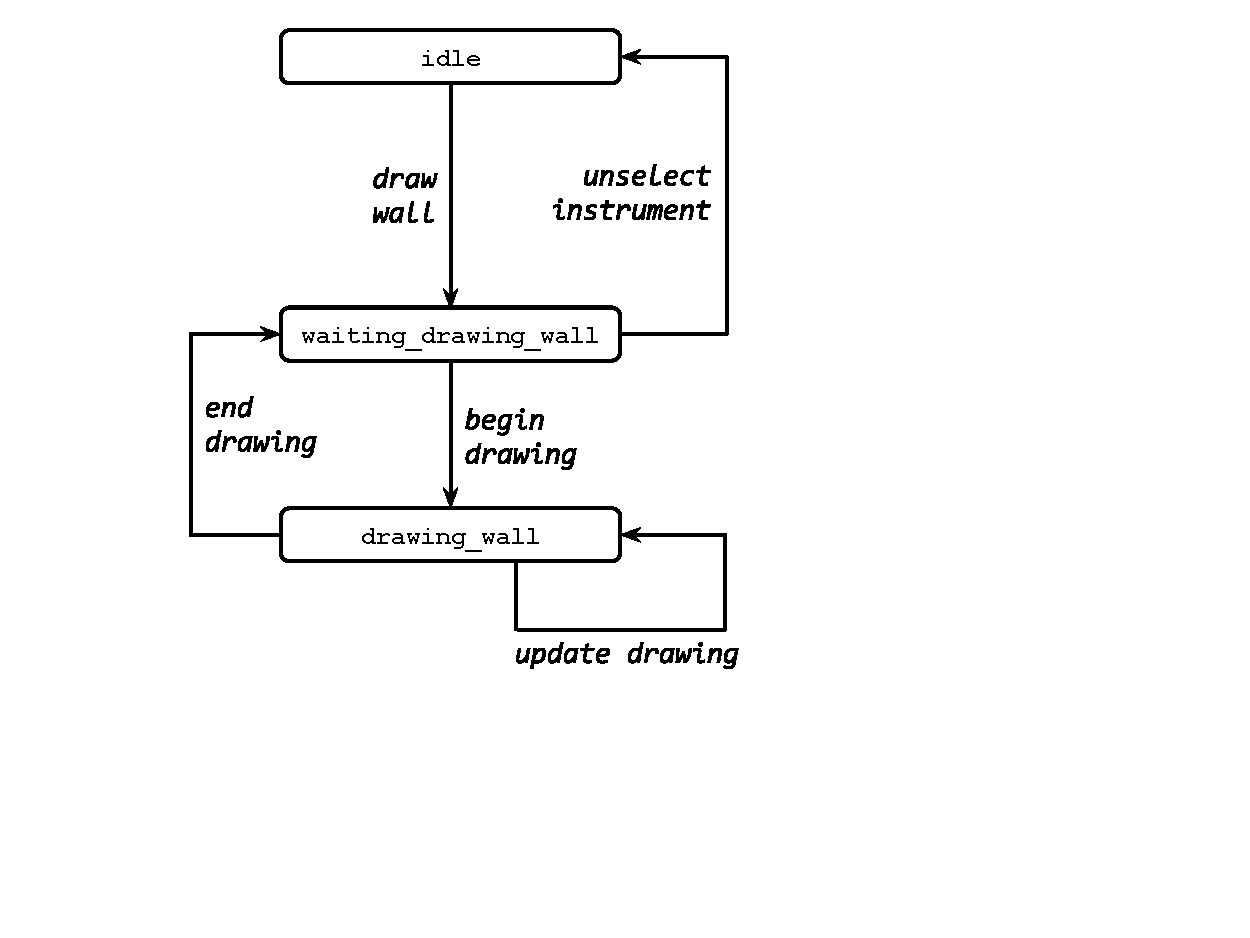
\includegraphics[width=0.6\linewidth]{contents/images/uc_draw_wall}

\caption{Subgraph of the state machine that show a wall creation.}
\label{fig_uc_draw_wall}
\end{figure}

\subsection{Component Based UI}


The entire application has been developed using separated modules, following the \textbf{SOLID programming} principles, as it could be expanded. For the web part, we have used the \textbf{web components pattern}, with the implementation of \textbf{React.js}\footnote{https://github.com/facebook/react} written by Facebook. The main idea is to define the frontend application as a collection of components, each one rendered in a different way according with values assigned to the state. In Figure~\ref{fig_ui} se can see the user interface of the application with the most interesting components: the toolbar (where every button is another component), the sidebar and the 2D viewer:

we have an example of based on our application.\\

\begin{figure}[h]
\centering
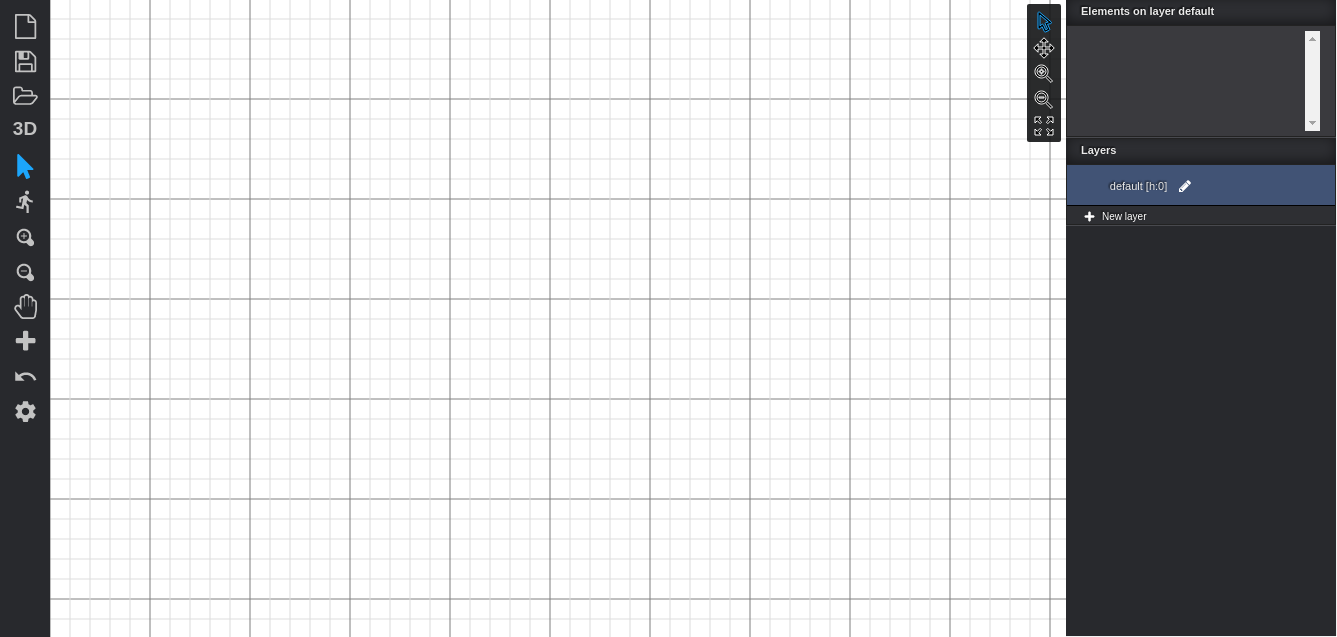
\includegraphics[width=\linewidth]{contents/images/ui}\\
\caption{User interface of the application}
\label{fig_ui}
\end{figure}

In particular, the most interesting components developed by us are the \textbf{viewers}, for example the 2D-viewer and the 3D-viewer. This component-based structure, allows us to define whatever state definition (for example in a tabular form) simply adding a new component.\\

The viewers structure is outlined in figure~\ref{fig_viewers}, where we can observe the great blocks. The first one is the \textit{catalog} and as we have already seen in section~\ref{building_elements} it contains all the building elements with their properties. We also see the application \textit{core}, which manages the state and contains all drawing functionalities, and can instantiate several different viewers giving them the state for the representation. It communicates with the catalog taking the building models properties. At least we have the \textit{viewers}, that are chosen observing the current state mode (see section~\ref{sec:central_state}). At the moment we implemented the 2D and 3D viewers (see figure~\ref{fig_viewer})\\\\
\textbf{2D Viewer}. This viewer creates a 2D view of the building model. Given the state, it exploit the \textbf{Virtual DOM} (see~\cite{vdom}) implemented by React.js, to update only changed parts avoiding continuously global updates. All elements are rendered using SVG DOM tag. To perform pan and zoom operations, typically necessary in this kind of tool, we used ReactSVGPanZoom~\footnote{https://github.com/chrvadala/react-svg-pan-zoom} a React component that adds pan and zoom features to SVG and helps to display big SVG images in a small space. It use affine matrix Math and event browser detection to adjust the image size to the required scale.\\\\
\textbf{3D Viewer}. It exploits the WEBGL-based modeling library \textbf{Three.js}~\footnote{https://threejs.org/} to build a 3D view of our building. To avoid global refreshes every time we update a part of the state, it has been implemented a \texttt{diff} and \textit{patch} system standardized in~\cite{rfc6902}. So it has been implemented a data structure that maps the Three.js objects with the building elements inside the state. Every time the user launches a Redux.js action, the application compute the difference between the old state and the new one a redraw only the changed objects. In particular we can have the following \textit{operations}: (i) \textbf{add}, (ii) \textbf{replace} and (iii) \textbf{remove}. For every operation it is determined a behavior based on the changed building element, changing also related building elements.

\begin{figure}[htb]
\centering
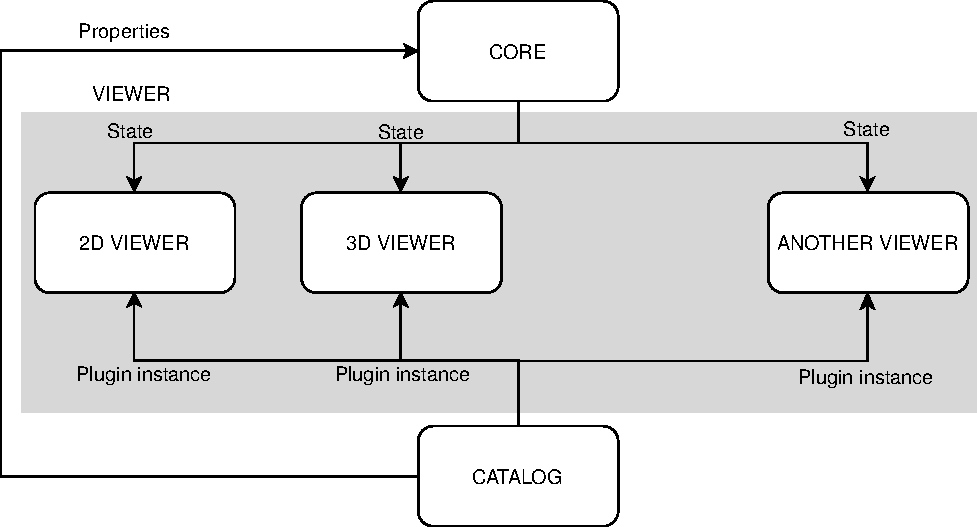
\includegraphics[width=\linewidth]{contents/images/diagramma-visualizzatori}

\caption{The architectural schema for the viewers}
\label{fig_viewers}
\end{figure}

\begin{figure}[htb]
\centering
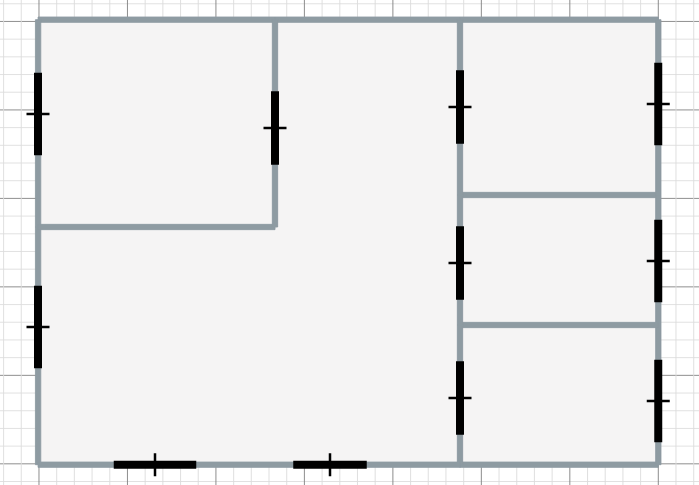
\includegraphics[width=0.45\linewidth]{contents/images/2d-viewer}
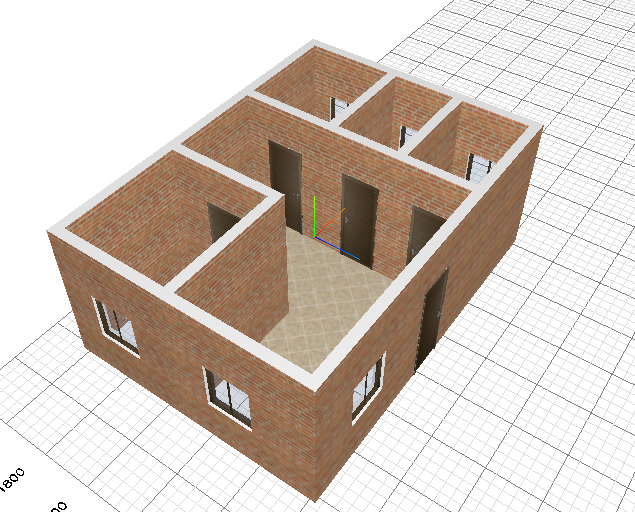
\includegraphics[width=0.45\linewidth]{contents/images/3d-viewer}
\caption{The 2D and 3D viewers for the state}
\label{fig_viewer}
\end{figure}